\section{Resultados y Discusiones}

En esta sección se presentarán los resultados obtenidos y se describirá la metodología aplicada para la optimización granulométrica de la mezcla entregada. Además, se analizarán dichos resultados para evaluar la efectividad del desarrollo. A continuación, se presentan los datos iniciales de las especificaciones de la mezcla.

\begin{table}[H]
\centering
\caption{Especificaciones de la mezcla de hormigón asignada.}
\begin{tabular}{|l|l|}
\hline
\textbf{Resistencia} & G15 \\ \hline
\textbf{Probabilidad defectuoso} & 1\% \\ \hline
\textbf{TMA} & 9,5 \\ \hline
\textbf{Elemento a hormigonar} & Fundación \\ \hline
\textbf{Condiciones de ejecución en obra} & Buenas \\ \hline
\textbf{Tipo de cemento} & Melón Extra \\ \hline
\textbf{Clase de exposición de la obra} & C0 \\ \hline
\textbf{Arena} & Arena 3 \\ \hline
\textbf{Gravilla} & Gravilla 2 \\ \hline
\textbf{Grava} & Grava 1 \\ \hline
\end{tabular}
\end{table}

\begin{table}[H]
\centering
\caption{Propiedades de los áridos utilizados.}
\begin{tabular}{|l|c|c|c|}
\hline
\textbf{Propiedad} & \textbf{Grava 1} & \textbf{Gravilla 2} & \textbf{Arena 3} \\ \hline
Absorción (\%)              & 1,30 & 1,20 & 1,20 \\ \hline
Humedad (\%)                & 4,00 & 8,00 & 6,00 \\ \hline
Peso específico (g/cm$^3$)  & 2,6  & 2,8  & 2,7  \\ \hline
Densidad (kg/m$^3$)         & 2600 & 2800 & 2700 \\ \hline
\end{tabular}
\end{table}

\subsection{Tamaño máximo de árido (TMA)}

Para esta parte del taller, se siguió la NCh 163, la cual establece los requisitos generales para los áridos en morteros y hormigones. Esta norma contiene los parámetros máximos de agregado que pueden estar presentes en una mezcla, según su uso estructural y características.

En primer lugar, se graficaron las curvas granulométricas de la Grava 1, Gravilla 2, Arena 3 y la Combinada, esta última es la ponderación de cada agregado con un parámetro inical de porcentaje a utilizar antes de optimizar. El gráfico se puede ver en la siguiente figura. Cabe mencionar que el tamizado con los resultados se presenta en la sección de Anexos.

\begin{table}[H]
\centering
\caption{Ponderaciones iniciales de los áridos para curva combinada.}
\begin{tabular}{|l|c|}
\hline
\textbf{Material} & \textbf{Ponderación Inicial (\%)} \\ \hline
Grava 1     & 20 \\ \hline
Gravilla 2  & 30 \\ \hline
Arena 3     & 50 \\ \hline
\end{tabular}
\end{table}


%Comenzar figura centrada
\begin{figure}[H]
    \centering
    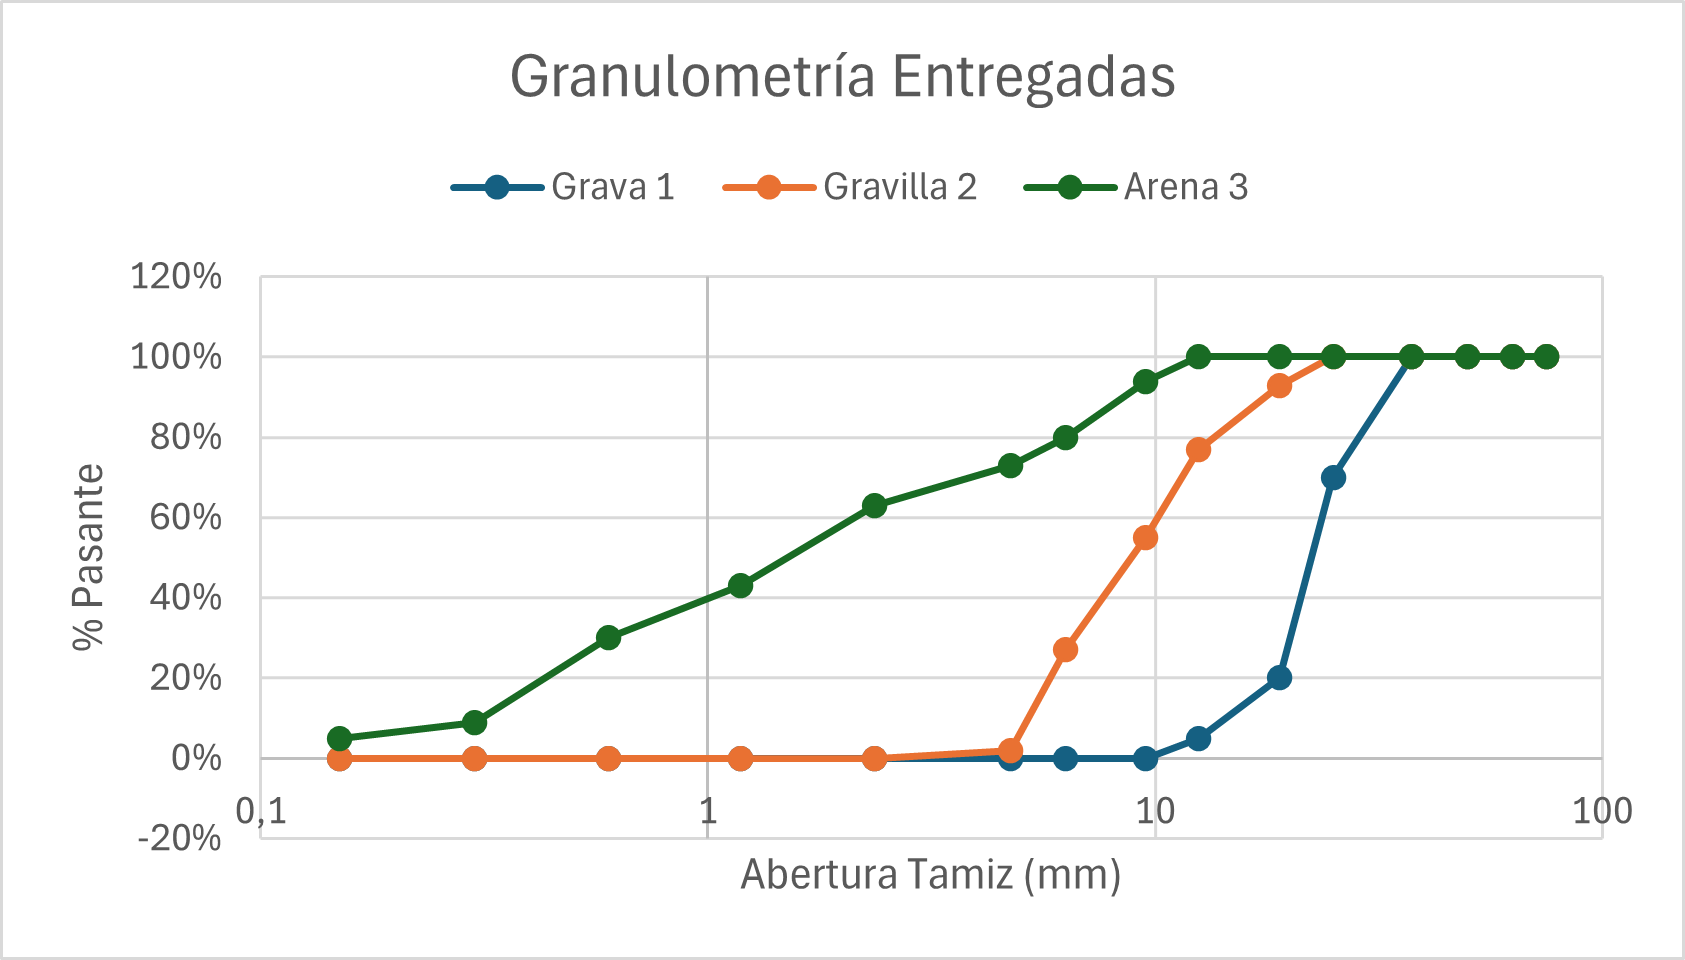
\includegraphics[width=0.8\textwidth]{GRAFICOS/granu_inicial.png}
    \caption{Curvas granulométricas iniciales de los áridos.}
\end{figure}

Posteriormente, en base a la norma, se graficaron las curvas asociadas al Dm 10mm, ya que por condición inicial el TMA es 9,5mm y se obtuvo la curva de granulometría sugerida, la cual es el promedio entre las curvas A, B, C y D. La figura se muestra a continuación.

\begin{figure}[H]
    \centering
    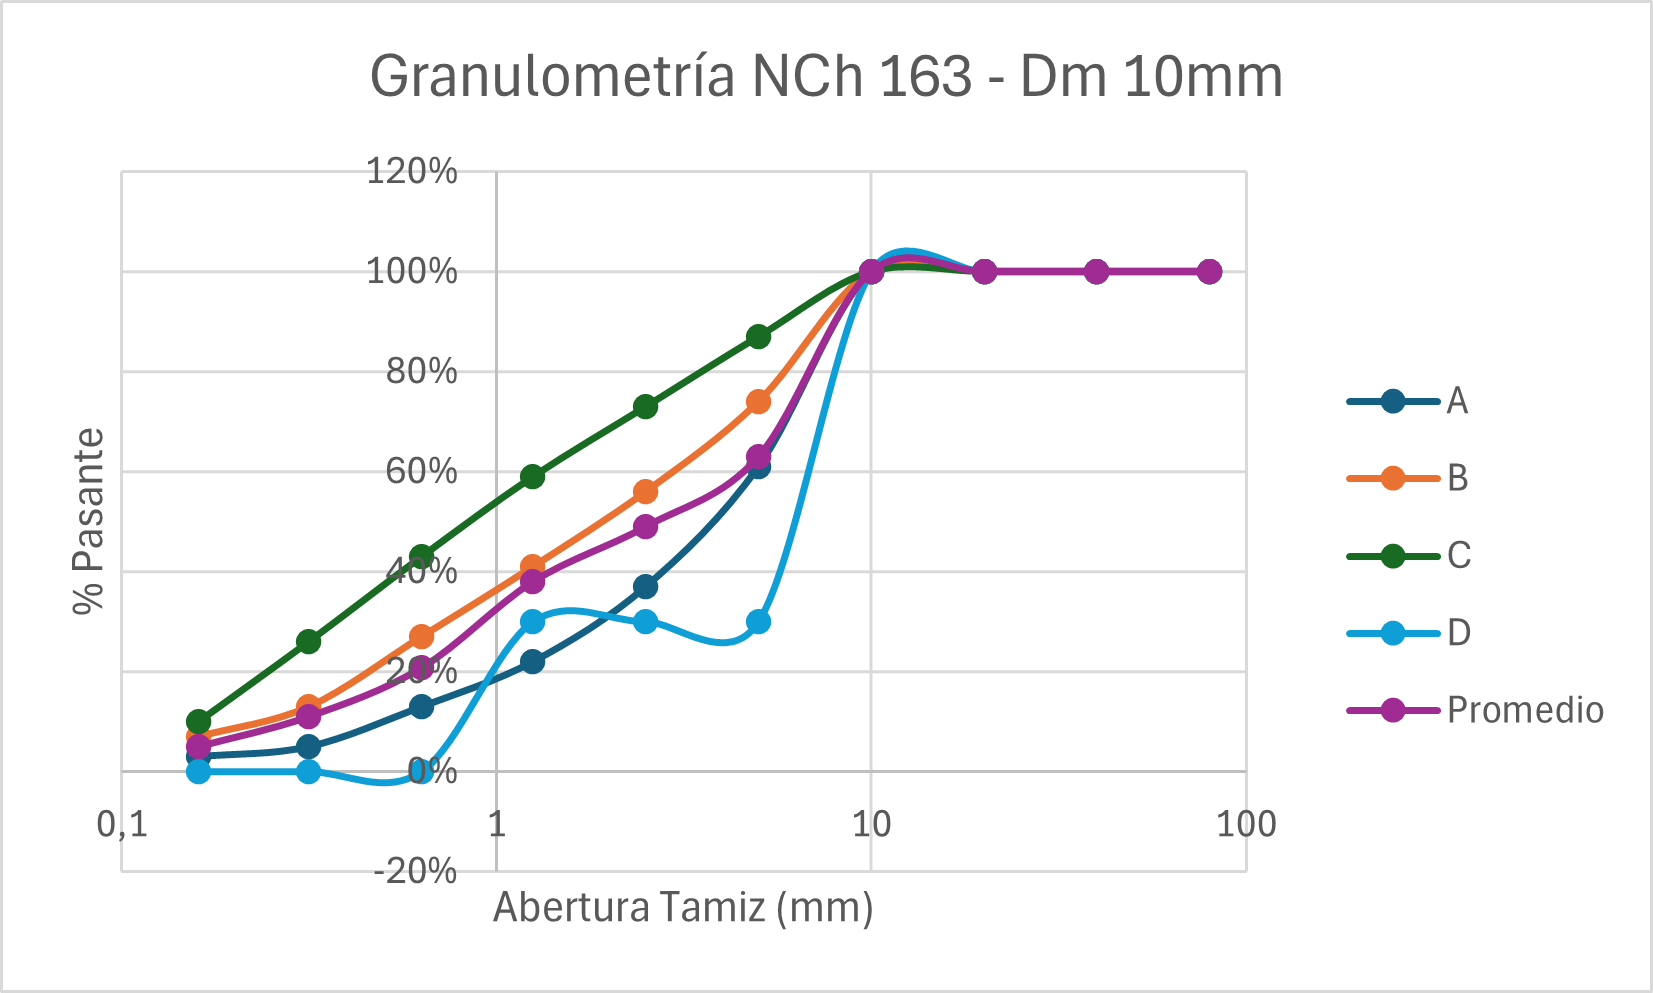
\includegraphics[width=0.8\textwidth]{GRAFICOS/NCh163.png}
    \caption{Curva de granulometría sugerida para Dm 10mm.}
\end{figure}

Una vez obtenida la curva sugerida, se procede a la optimización granulométrica en base a la norma. Este proceso consistió en interpolar los \% pasantes combinados de nuestra mezcla a los tamices indicados en la norma para poder compararlos. Finalmente, se realizó una iteración con la función objetivo de Excel para poder llevar la curva combinada a la sugerida, la cual varía los \% de cada árido hasta que la diferencia entre ambas curvas sea igual a 0, lo que da como resultado la curva optimizada.

La siguiente tabla muestra los \% finales obtenidos para la ponderación de cada árido y la figura muestra la curva optmizada comparada con la curva sugerida. Se puede notar que la diferencia entre ambas esta minimizada.

\begin{table}[H]
\centering
\caption{Ponderaciones finales de los áridos utilizando método de Banda.}
\begin{tabular}{|l|c|}
\hline
\textbf{Material} & \textbf{Ponderación Final (\%)} \\ \hline
Grava 1     & 0 \\ \hline
Gravilla 2  & 7 \\ \hline
Arena 3     & 93 \\ \hline
\end{tabular}
\end{table}

\begin{figure}[H]
    \centering
    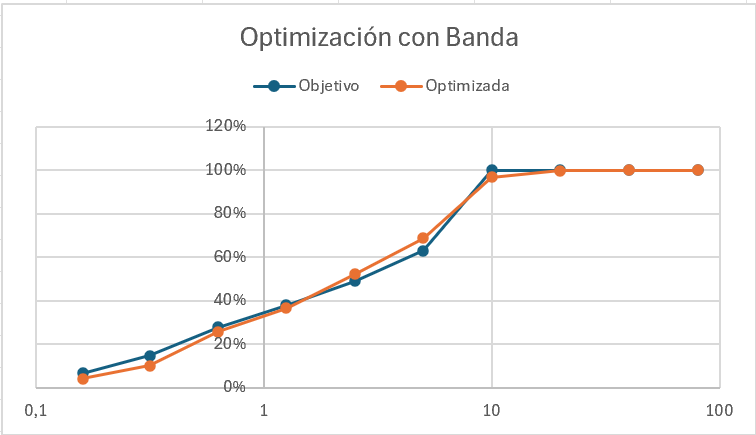
\includegraphics[width=0.8\textwidth]{GRAFICOS/opti_banda.png}
    \caption{Curva granulométrica optimizada comparada con la curva sugerida.}
\end{figure}

Dadas las condiciones iniciales, las condiciones de ejecución en obra, el elemento a hormigonar, el tipo de hormigón y la clase de exposición en obra, se llegó a una dosificación casi en su totalidad compuesta por arena, con un pequeño porcentaje de gravilla, destacando la nula presencia de grava. Además, se obtuvieron las proporciones de los otros compuestos como cemento y agua con sus respectivas correcciones por humedad. La siguiente tabla muestra los resultados finales.

\begin{table}[H]
\centering
\caption{Dosificación final con factores corregidos.}
\begin{tabular}{|c|c|c|c|c|} % Centrado vertical y horizontal en cada celda
\hline
\textbf{Material} & \textbf{Dosificación SSS $(kg/m^3)$} & \textbf{Agua interna $(kg)$} & \textbf{Peso seco $(kg)$} & \textbf{Dosificación Húmedos $(kg/m^3)$} \\ \hline
Cemento & 334,55 & - & - & 334,55 \\ \hline
Agua amasado & 177,98 & - & - & 85,27 \\ \hline
Grava 1 & 0 & 0 & 0 & 0 \\ \hline
Gravilla 2 & 124,98 & 9,88 & 123,05 & 133,38 \\ \hline
Arena 3 & 1777,46 & 105,38 & 1756,38 & 1861,77 \\ \hline
\end{tabular}
\label{tab:ejemplo}
\end{table}

\vspace{1cm}
\subsection{Fuller - Thompson}

En esta sección se realizó una nueva optimización granulométrica utilizando el método de Fuller-Thomposon. Esta curva sigue una distribución de potencia, como se expresa a continuación:

\begin{equation}
    P(D) = 100 \times (\frac{D}{D_{max}})^n
\end{equation}

Donde $P(D)$ es el \% que pasa por el tamiz de diámetro $D$, $D_{max}$ es el tamaño máximo del árido (TMA) y $n$ es el exponente que define la forma de la curva, el cual, según Fuller, tiene un valor de 0,45 para hormigones.

El objetivo es lograr que la curva de los áridos combinados con los \% optimizados sea lo más parecida a la curva sugerida por el método Fuller - Thompson, minimizando su diferencia. La curva sugerida se obtiene reemplazando la dosificación sugerida por la NCH 163 en la fórmula anterior.  

A continuación se muestran los resultados obtenidos.

\begin{table}[H]
\centering
\caption{Ponderaciones finales de los áridos utilizando Fuller-Thompson.}
\begin{tabular}{|l|c|}
\hline
\textbf{Material} & \textbf{Ponderación Final (\%)} \\ \hline
Grava 1     & 0 \\ \hline
Gravilla 2  & 5 \\ \hline
Arena 3     & 95 \\ \hline
\end{tabular}
\end{table}

\begin{figure}[H]
    \centering
    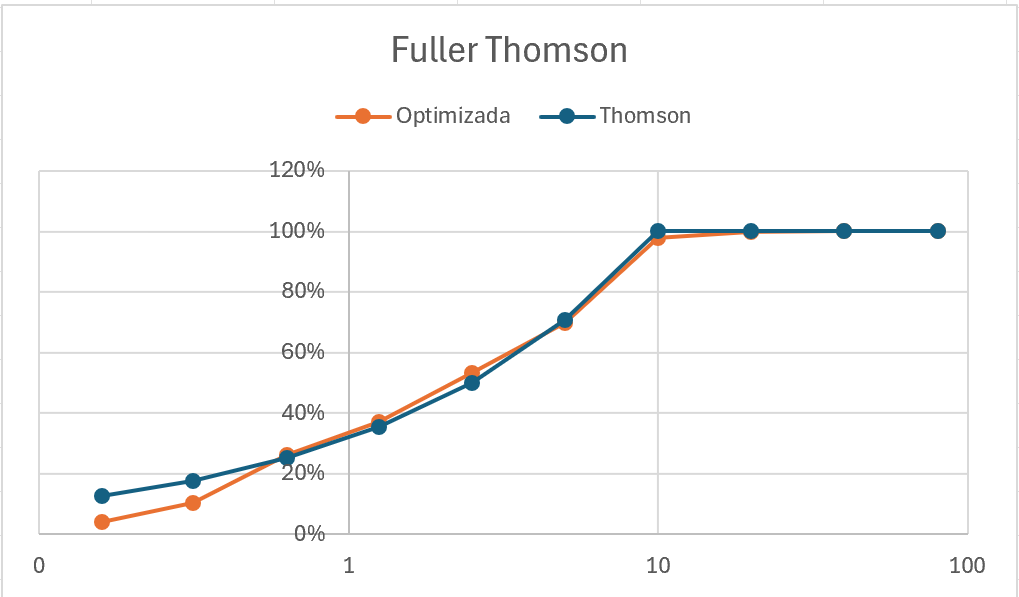
\includegraphics[width=0.8\textwidth]{GRAFICOS/fuller_thompson.png}
    \caption{Curva granulométrica optimizada comparada con la curva Fuller-Thompson.}
\end{figure}

Se puede analizar que los resultados son similares a los obtenidos por el método de Banda, donde hay nula presencia de gravas y un alto porcentaje de arena. Además, se puede observar que la diferencia de cada punto de la curva optimizada con la sugerida es mínima.

Posteriormente, se obtuvieron las masas requeridas de agua, cemento y agregados corregidas, utilizando las condiciones y requerimientos iniciales.

\begin{table}[H]
\centering
\caption{Dosificación final corregida por humedad.}
\begin{tabular}{|l|c|c|c|c|}
\hline
\textbf{Material} & 
\textbf{Dosificación SSS (kg/m$^3$)} & 
\textbf{Agua interna (kg)} & 
\textbf{Peso seco (kg)} & 
\textbf{Dosificación Húmedos (kg/m$^3$)} \\ \hline

Cemento   & 334,56 & -      & -       & 334,56 \\ \hline
Agua de amasado & 177,98 & -      & - & 86,10 \\ \hline
Grava 1   & 0,00   & 0,00   & 0,00   & 0,00 \\ \hline
Gravilla 2 & 86,74  & 6,86   & 85,71  & 92,57 \\ \hline
Arena 3   & 1814,34 & 107,57 & 1792,83 & 1900,40 \\ \hline
\end{tabular}
\end{table}


FALTA UN POCO MAS DE ANÁLISIS EN CADA PARTE







